\section{Multigrid Methods}
Multigrid methods have been designed to accelerate the convergence of iterative methods by eliminating certain error components on a so-called coarser representation of the original problem.
While the basic iterative methods discussed in the last section are applicable to many PDE-based problems, in practice, their speed of convergence is often insufficient, which means that a large number of iterations is required until an acceptable approximation accuracy can be attained. 
The main reason for this behavior is that these methods are only efficient in the reduction of certain error components, while others remain mostly unaffected~\cite{briggs2000multigrid}.
This can be best understood by considering the effect of a stationary iterative method on oscillatory errors of different frequency.
For this purpose, we consider the one-dimensional Laplace equation
\begin{equation}
		\begin{split}
			- \dv[2]{x} u(x) & = 0 \quad \forall x \in (0, 1) \\
			u(0) = u(1) & = 0,
		\end{split}
		\label{eq:1D-laplace-model}
\end{equation}
which is discretized using the three-point stencil
\begin{equation}
	\Delta_h^{(3, 1)} = \frac{1}{h^2}\begin{bmatrix}
		-1 & 2 & -1
	\end{bmatrix}.
\end{equation} 
Figure~\ref{fig:different-error-components-jacobi} shows the impact of applying the Jacobi´and Gauss-Seidel method on different periodic error components.
\begin{figure}
	\centering
	\begin{subfigure}[b]{0.32\textwidth}
		\centering
		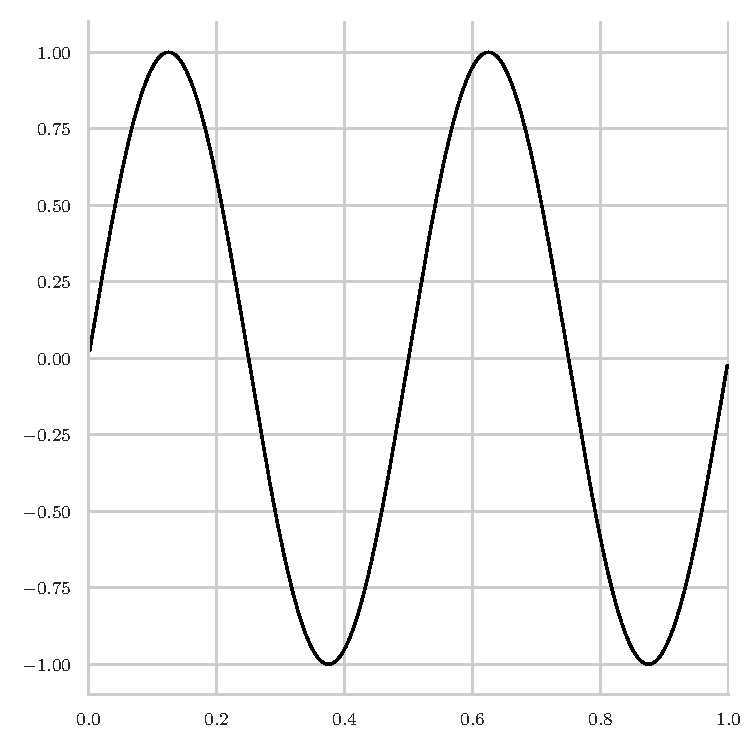
\includegraphics[width=\textwidth]{figures/initial_error_jacobi_4pi.pdf}
		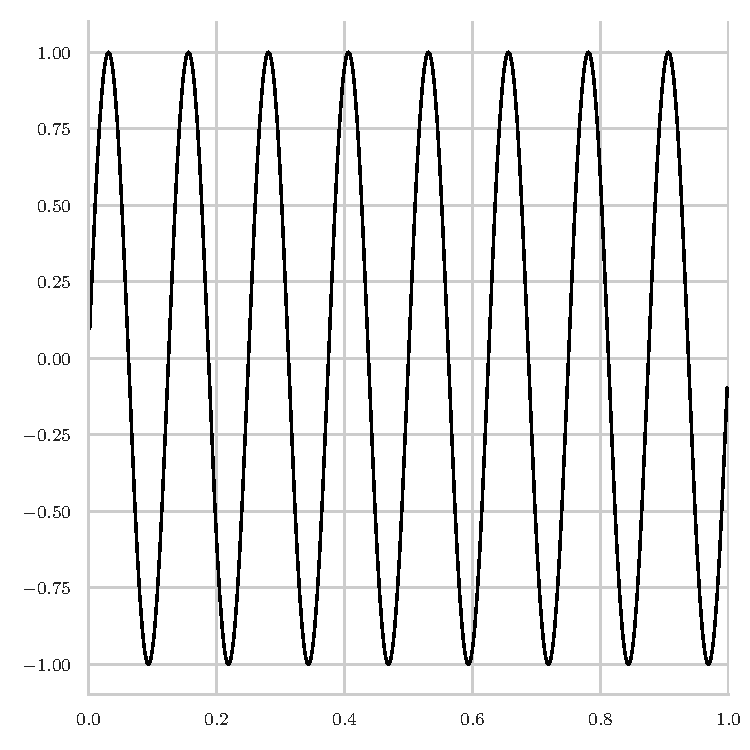
\includegraphics[width=\textwidth]{figures/initial_error_jacobi_16pi.pdf}
		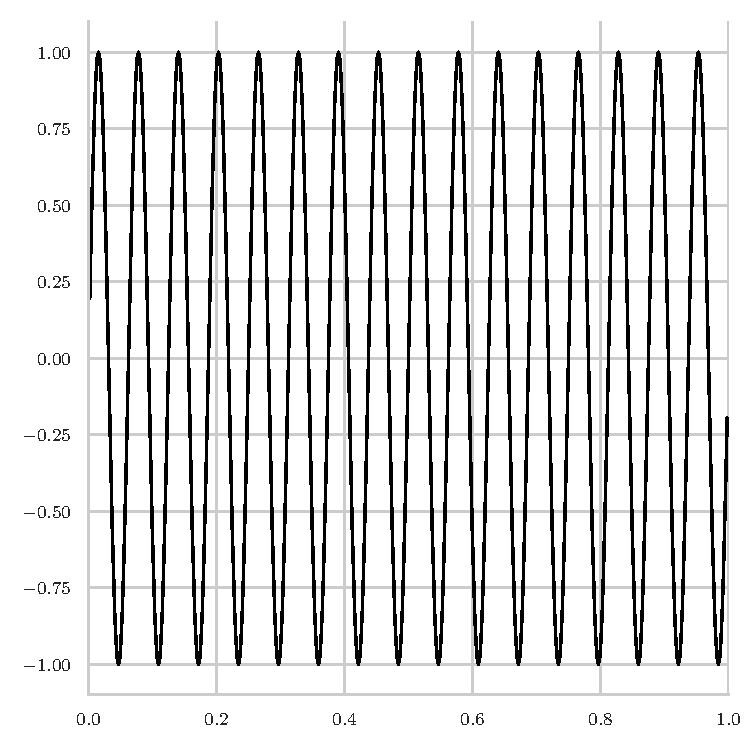
\includegraphics[width=\textwidth]{figures/initial_error_jacobi_32pi.pdf}
		\caption{Initial error}
	\end{subfigure}
	\hfill
	\begin{subfigure}[b]{0.32\textwidth}
		\centering
		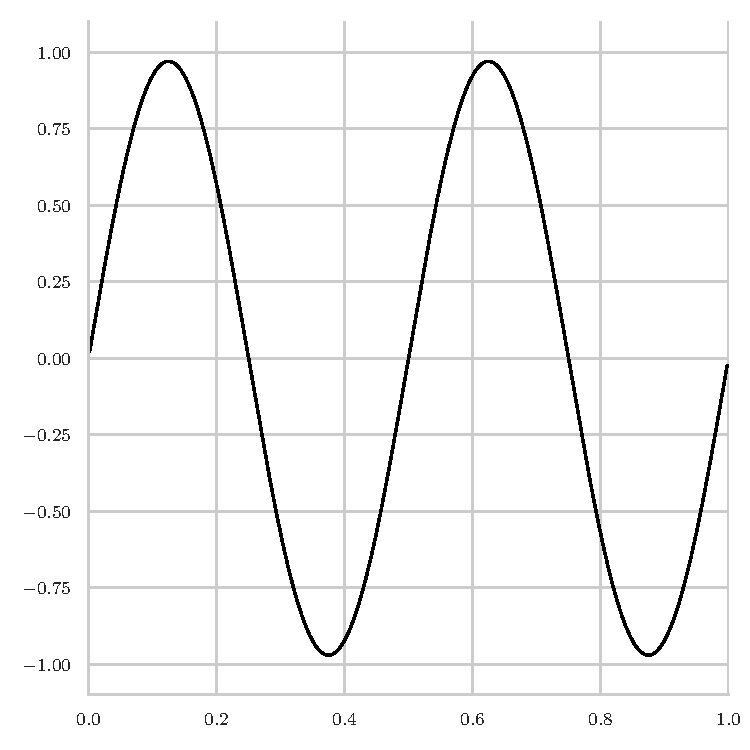
\includegraphics[width=\textwidth]{figures/final_error_jacobi_4pi.pdf}
		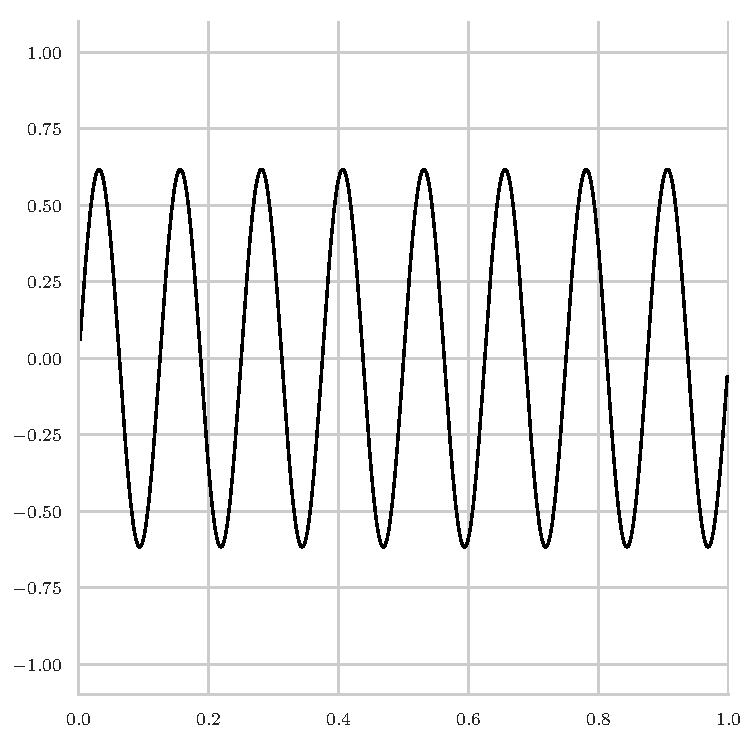
\includegraphics[width=\textwidth]{figures/final_error_jacobi_16pi.pdf}
		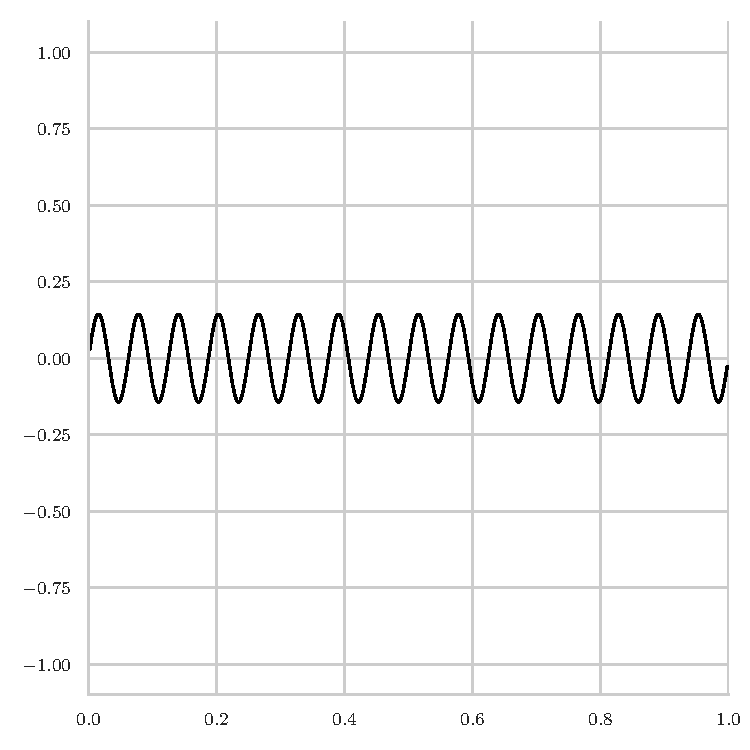
\includegraphics[width=\textwidth]{figures/final_error_jacobi_32pi.pdf}
	\caption{Error after applying Jacobi}
	\end{subfigure}
	\hfill
	\begin{subfigure}[b]{0.32\textwidth}
		\centering
		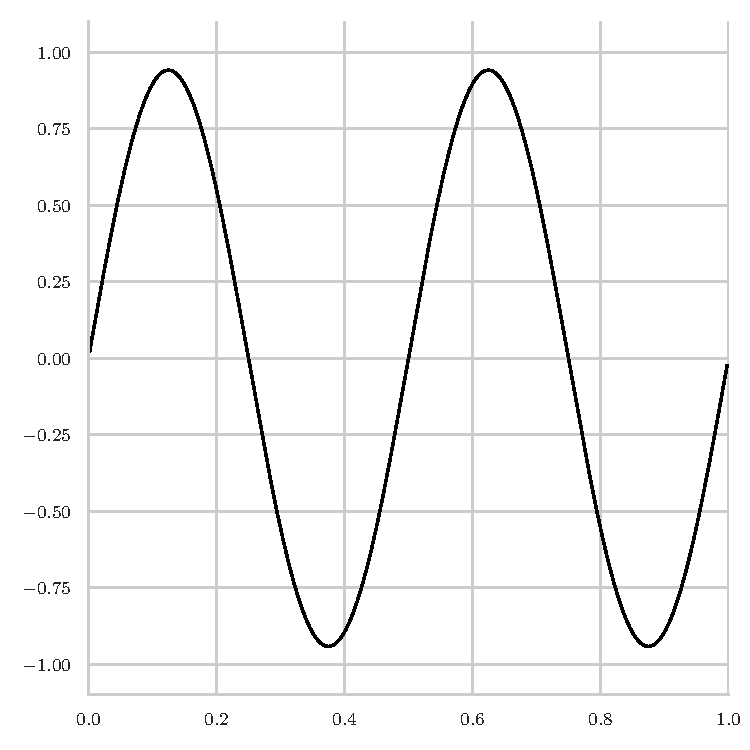
\includegraphics[width=\textwidth]{figures/final_error_gauss_seidel_4pi.pdf}
		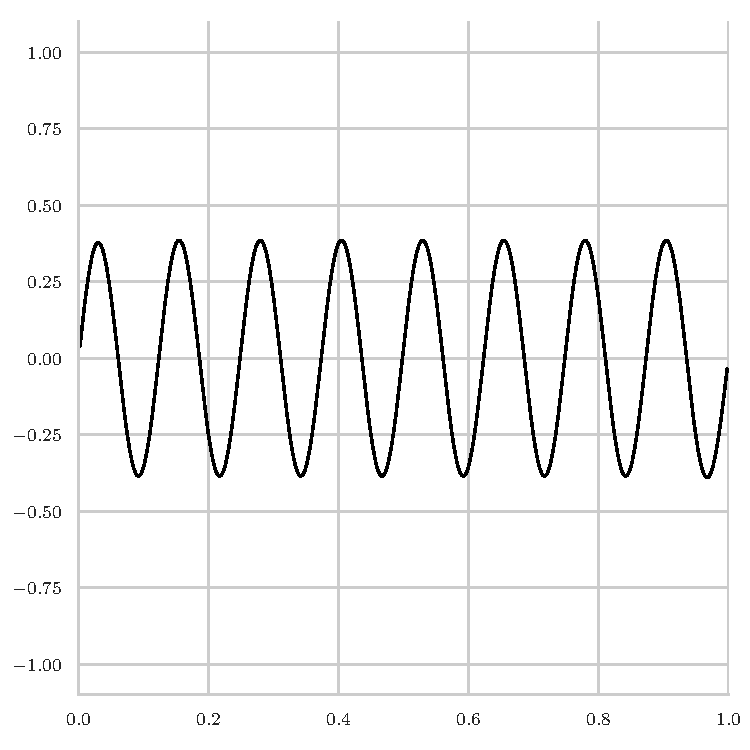
\includegraphics[width=\textwidth]{figures/final_error_gauss_seidel_16pi.pdf}
		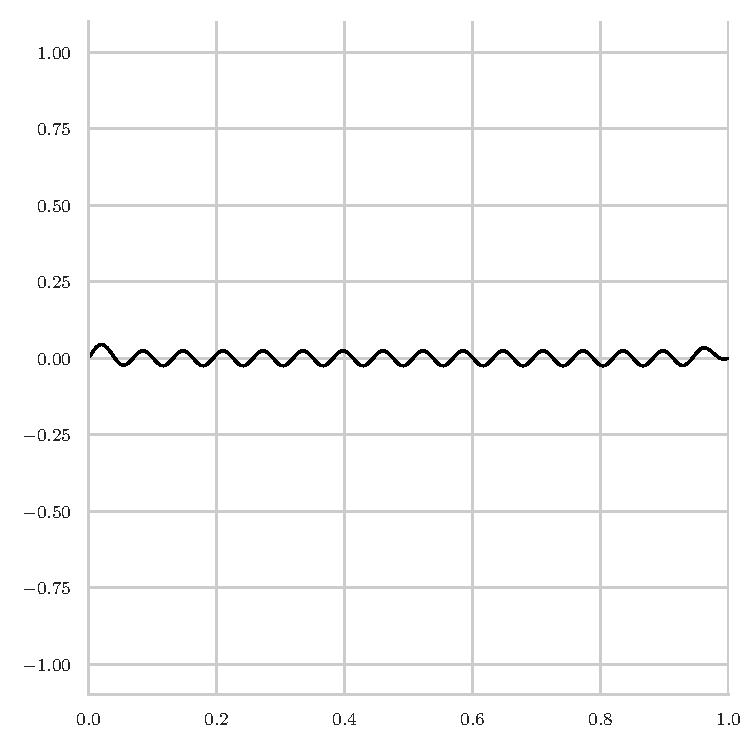
\includegraphics[width=\textwidth]{figures/final_error_gauss_seidel_32pi.pdf}
	\caption{Error after applying Gauss-Seidel}
	\end{subfigure}
	\caption{Different error components on a grid with step size $h = 2^{-9}$ before and after applying either 100 steps of the Jacobi or Gauss-Seidel method.}
	\label{fig:different-error-components}
\end{figure}
Here, the left column shows the initial error discretized on a grid with step size $h = 2^{-9}$ while the middle and right one includes the remaining error after applying 100 Jacobi and Gauss-Seidel steps, respectively.
Note that the frequency of change increases from top to bottom, whereas the amplitude of the error is always the same.
As it becomes apparent from investigating the middle and right columns of the first row of Figure~\ref{fig:different-error-components}, the Jacobi and Gauss-Seidel methods are both not able to achieve a significant reduction of those error components with a low frequency of change within 100 iterations.
In contrast, the third row, which represents a highly-oscillating component, the application of 100 steps of the Jacobi method already reduces the initial error to less than one-fifth of its original value.
The same behavior can also be observed for the Gauss-Seidel method, whereby, compared to the Jacobi method, high-frequency error components are reduced even faster.

We can further illustrate the error reduction properties of basic iterative methods by investigating Figure~\ref{fig:combined-error} which shows the combination of two error components with equal magnitude, one of them with low, the other one with high frequency.
Again, the left plot shows the initial while the right one contains the reduced error after 100 iterations of Jacobi.
As it can be seen here, the attained improvement can be almost fully attributed to the reduction of the highly-oscillating component.
\begin{figure}
	\begin{subfigure}[b]{0.32\textwidth}
	\centering
		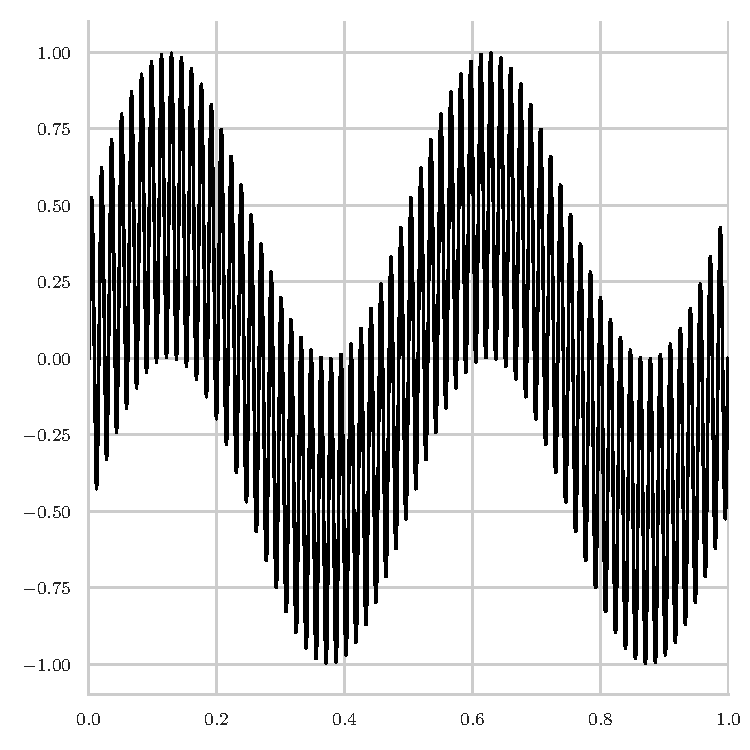
\includegraphics[width=\textwidth]{figures/initial_error_jacobi_combined.pdf}
		\caption{Initial error}
\end{subfigure}
\hfill
\begin{subfigure}[b]{0.32\textwidth}
	\centering
		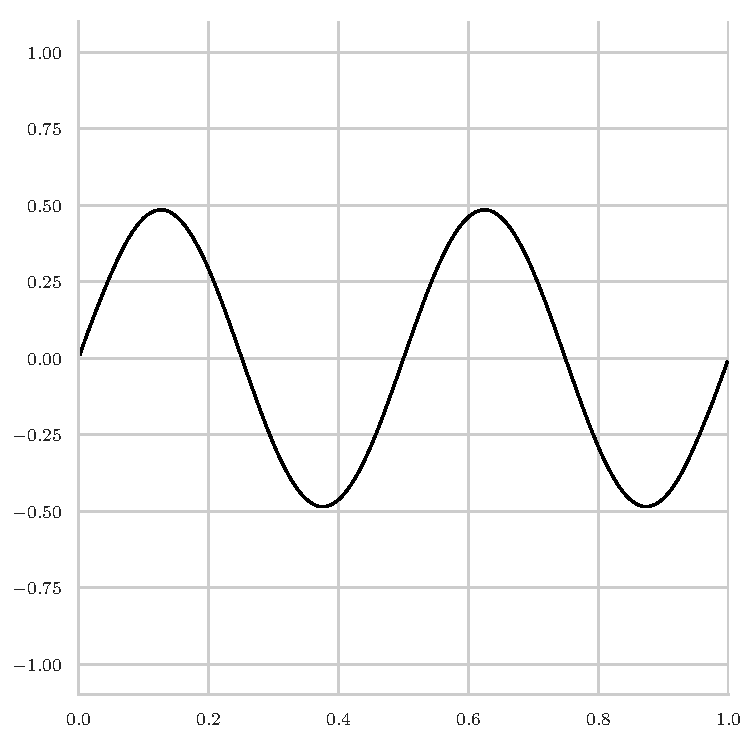
\includegraphics[width=\textwidth]{figures/final_error_jacobi_combined.pdf}
		\caption{Error after applying Jacobi}
\end{subfigure}
\begin{subfigure}[b]{0.32\textwidth}
	\centering
	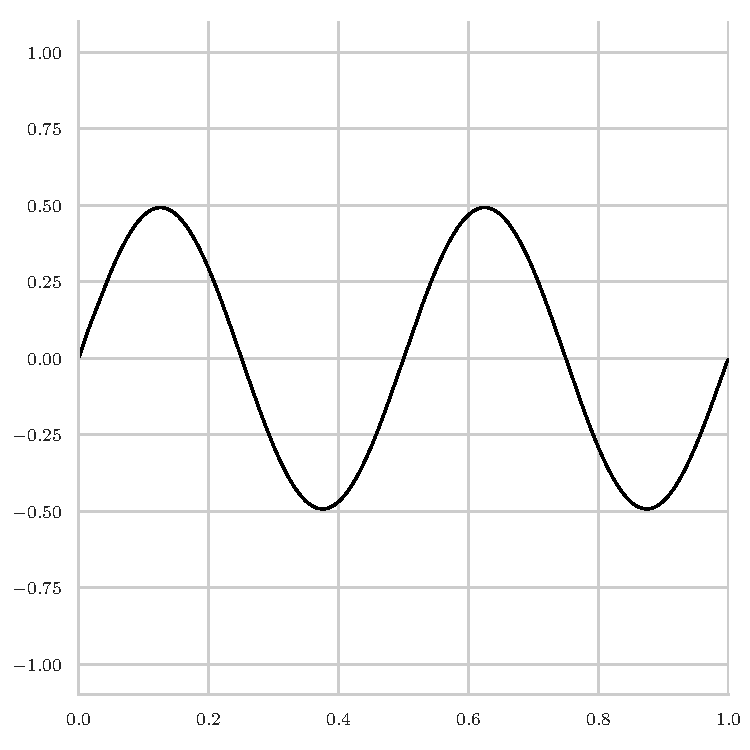
\includegraphics[width=\textwidth]{figures/final_error_gauss_seidel_combined.pdf}
	\caption{Error after applying Gauss-Seidel}
\end{subfigure}
	\caption{Combination of two error components discretized on a grid with step size $h = 2^{-9}$ before and after applying 100 steps of either the Jacobi or Gauss-Seidel method.}
\label{fig:combined-error}
\end{figure}

Now observe what happens if we represent the same low-frequency error component shown in the first row of Figure~\ref{fig:different-error-components} on a grid with larger step size $h = 2^{-6}$, hence a smaller number of grid points.
\begin{figure}
	\begin{subfigure}[b]{0.32\textwidth}
	\centering
	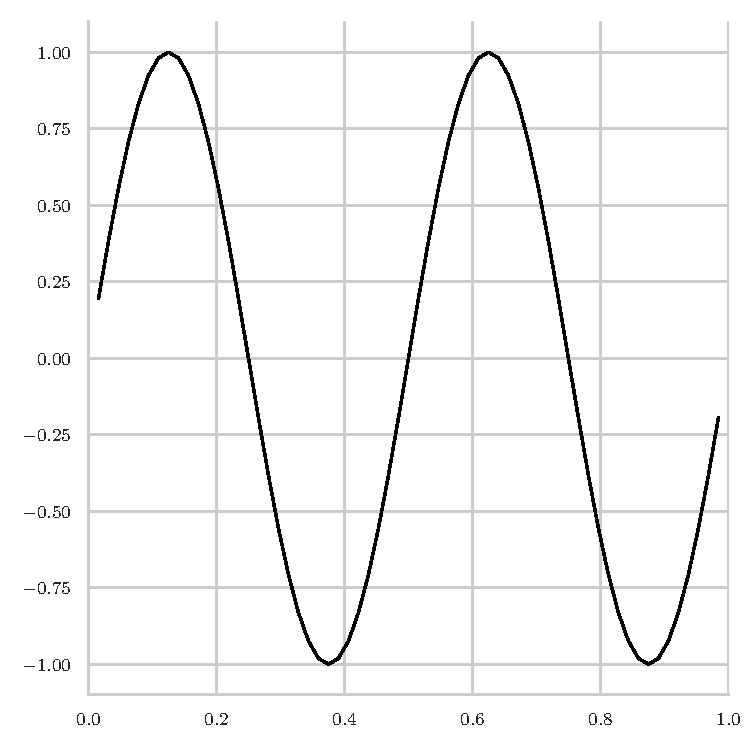
\includegraphics[width=\textwidth]{figures/initial_error_jacobi_4pi_coarse.pdf}
	\caption{Initial error}
\end{subfigure}
\hfill
\begin{subfigure}[b]{0.32\textwidth}
	\centering
	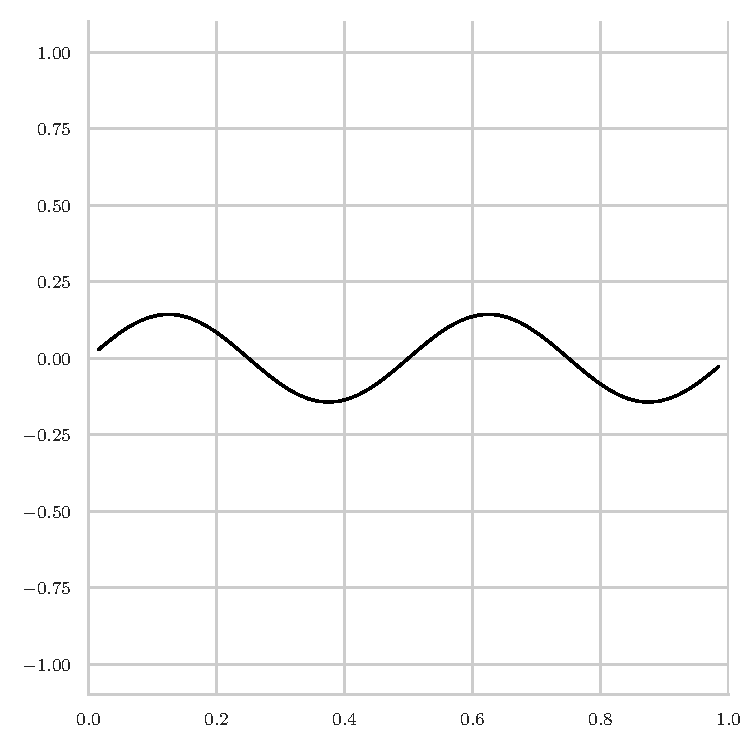
\includegraphics[width=\textwidth]{figures/final_error_jacobi_4pi_coarse.pdf}
	\caption{Error after applying Jacobi}
\end{subfigure}
	\hfill
	\begin{subfigure}[b]{0.32\textwidth}
		\centering
		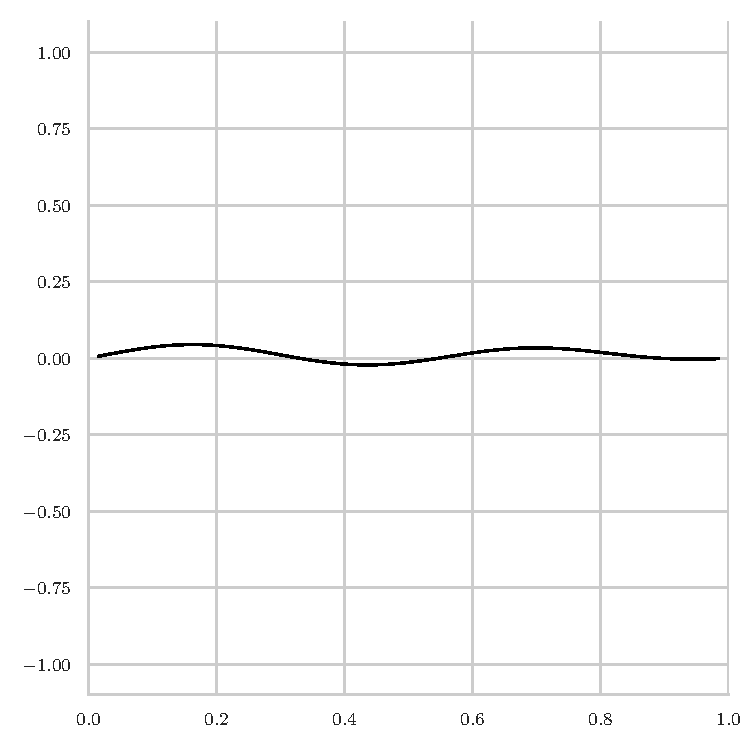
\includegraphics[width=\textwidth]{figures/final_error_gauss_seidel_4pi_coarse.pdf}
		\caption{Error after applying Gauss-Seidel}
	\end{subfigure}
	\caption{Low-frequency error component discretized on a coarse grid with step size $h = 2^{-6}$ before and after applying 100 steps of either the Jacobi or Gauss-Seidel method.}
	\label{fig:low-frequency-error-component-coarse}
\end{figure}
